\documentclass{standalone}
\usepackage{tikz}
\usetikzlibrary{calc}
\begin{document}
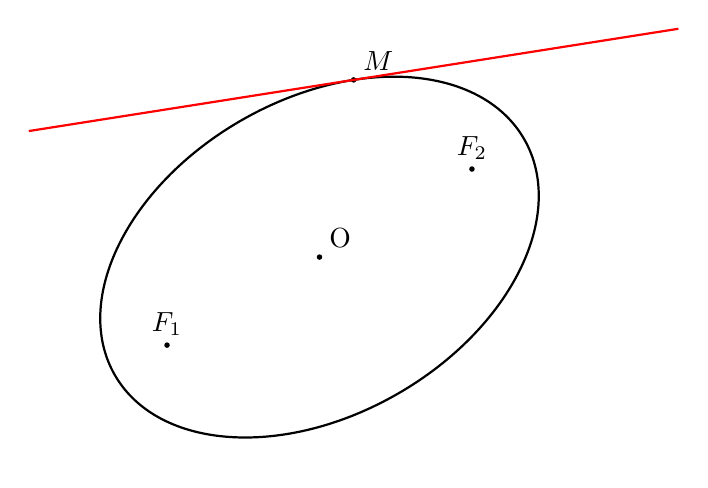
\begin{tikzpicture}
\def\xC{8}
\def\yC{3}
\def\a{3}
\def\b{2}
\def\ang{30}
% Draw axes
%\draw[->] (-1,0) -- (15,0) node[below] {$x$};
%\draw[->] (0,-1) -- (0,6) node[left] {$y$};

% Ellipse
\draw[thick, rotate around={\ang:(\xC,\yC)}] (\xC,\yC) ellipse [x radius=\a, y radius=\b];

% Center
\fill (\xC,\yC) circle (1pt) node[above right] {O};

% Foci
\pgfmathsetmacro{\c}{sqrt(\a*\a - \b*\b)}
\coordinate (F1) at ({\xC+\c*cos(\ang)},{\yC+\c*sin(\ang)});
\coordinate (F2) at ({\xC-\c*cos(\ang)},{\yC-\c*sin(\ang)});
\fill (F2) circle (1pt) node[above] {$F_1$};
\fill (F1) circle (1pt) node[above] {$F_2$};

% ---- Tangent at a point ----
% Choose a point on the ellipse using parametric angle t (0-360 degrees)
\def\t{60} % parametric angle in degrees (ellipse before rotation)

% Coordinates of point before rotation
\pgfmathsetmacro{\xP}{\xC + \a*cos(\t)}
\pgfmathsetmacro{\yP}{\yC + \b*sin(\t)}

% Rotate point by ellipse angle
\pgfmathsetmacro{\xPR}{\xC + (\xP-\xC)*cos(\ang) - (\yP-\yC)*sin(\ang)}
\pgfmathsetmacro{\yPR}{\yC + (\xP-\xC)*sin(\ang) + (\yP-\yC)*cos(\ang)}

% Draw the point
\fill (\xPR,\yPR) circle (1pt) node[above right] {$M$};

% Tangent vector at P (parametric derivative)
\pgfmathsetmacro{\dx}{-\a*sin(\t)}
\pgfmathsetmacro{\dy}{\b*cos(\t)}

% Rotate derivative vector
\pgfmathsetmacro{\dxR}{\dx*cos(\ang) - \dy*sin(\ang)}
\pgfmathsetmacro{\dyR}{\dx*sin(\ang) + \dy*cos(\ang)}

% Draw tangent line
\draw[red, thick] 
    ($(\xPR,\yPR)+(-1.5*\dxR,-1.5*\dyR)$) -- 
    ($(\xPR,\yPR)+(1.5*\dxR,1.5*\dyR)$);
\end{tikzpicture}
\end{document}